\documentclass[12pt,twoside=off,
bibtotoc,liststotoc,appendixprefix,paper=a4,headings=small]{scrbook} % 'twoside=on' für Druckversion oder 'twoside=off' für Onlineversion

\makeatletter
\renewcommand\chapter{\thispagestyle{plain}%
\global\@topnum\z@
\@afterindentfalse
\secdef\@chapter\@schapter}
\makeatother

%
% Packages
% -----------------------------------
\usepackage{scrhack}                  % Fixes deprecated \float@addtolist warning in KOMA-Script
\usepackage[
  paper=a4paper,
  left=12.5mm,
  right=25mm,
  top=25mm,
  bottom=50mm,
  bindingoffset=10mm]{geometry}		% Seitenränder und Bindungskorrektur einstellen
  
\usepackage{apacite} 				% Literatur-Referenzen: American Psycholog. Assoc.
\usepackage[utf8]{inputenc}         % Umlaute im Text
\usepackage{ngerman}				% Rechtschreibg.
\usepackage[T1]{fontenc}
\usepackage{lmodern}				% Schriftfamilie
\setkomafont{disposition}{\bfseries}

\usepackage{graphicx} 				% Grafiken einfügen (pdf,png - aber jpg vermeiden)
\graphicspath{{./Bilder/}}          % Pfad zu den Bildern

\usepackage{url}					% URL's formatieren (z.B. in Literatur) 
\usepackage[colorlinks,linkcolor=black,citecolor=black,urlcolor=black]{hyperref} 				% für Hyperlinks in PDF-Dokumenten   
  
\usepackage{tabularx} 				% bessere Gestaltung von Tabellen
\usepackage{longtable} 		
\usepackage{multicol}				
\usepackage{multirow}
\usepackage{booktabs}
\usepackage{tabularx}
		
\usepackage[active]{srcltx}

\usepackage{listings}				% Algorithmen

\usepackage{mdwlist}				% Listen
\usepackage{enumitem}               % Customizable lists

\usepackage{setspace} 				% Zeileneinstellung
\newtheorem{mydef}{Merksatz}  		% Falls Beispiele, Merksätze m. fortl. Nr. gebr. werden
\newtheorem{bsp}{Beispiel}

\usepackage{lscape}					% zum Rotieren von Seiten

\usepackage{amsmath}				% zum Schreiben von mathematischen Formeln
\usepackage{float}                  % für [H] Platzierungsoption bei Figures

\usepackage{calc}

\usepackage{footnote}				% Fußnoten (entfernt wegen Konflikt mit microtype)
\usepackage{tablefootnote}			% Fußnoten in Tabellen
\usepackage{cleveref}
%\clubpenalty = 10000
%\widowpenalty = 10000 \displaywidowpenalty = 10000

\hyphenation{voll-st\"andigen}		% Worttrennungen global definieren

\setcounter{tocdepth}{1}			% Ebenen, die im Inhaltsverzeichnis angezeigt werden

% Document
% -----------------------------------
\begin{document}

\frontmatter 
    % Titelseite soll keine Kopf oder Fußzeile haben
\thispagestyle{empty}

% Alle Elemente sollen zentriert sein
\begin{center}

\vspace*{-10mm}

{\LARGE FACHBEREICH \\WIRTSCHAFTSWISSENSCHAFTEN\\[1mm]}
DER FREIEN UNIVERSITÄT BERLIN\\

\vspace*{1cm}


\includegraphics[width=0.18\textwidth]{fu_logo}

\vspace*{1cm}

% Art der Arbeit => (Bachelorarbeit ,Diplomarbeit, Masterarbeit, Seminararbeit)
{\Large \textbf{Seminararbeit}}\\ 

\vspace{1cm}

% Titel der Arbeit 
{\Large \textbf{The Economic Relationship}}\\ 
\vspace*{1mm}
{\Large \textbf{between China and Russia}}\\ 
\vspace*{1mm}
{\Large \textbf{before and after the Russia-Ukraine War}}\\

\vspace{1.5cm}

% Name des/der Autors/Autoren
{\LARGE Katharina Hansen}\\[15mm]

% Gutachter, Kontaktdaten und Abgabetermin
\parbox{120mm}{
\begin{large}
\begin{tabbing}
Gutachter: \hspace{.7cm} \=Prof. Dr. Laike Yang\\[4mm]
Semester:\> Sommersemester 2025\\
Verfasser:\> Katharina Hansen\\ % alphabetische Reihenfolge (Nachname)
Matrikel-Nr.:\> 5576002\\
Email:\> katharih04@zedat.fu-berlin.de\\
Studienfach:\>Bachelor VWL\\[8mm]
\end{tabbing}
\end{large}
}

\end{center}
\clearpage{\pagestyle{empty}\cleardoublepage}
 			% Titelblatt
    \clearpage{\pagestyle{empty}\cleardoublepage}
    \onehalfspacing                  	% Zeilenabstand ab hier 1.5 zeilig
    \tableofcontents 					% Inhaltsverzeichnis
    \clearpage{\pagestyle{empty}\cleardoublepage} 
% -----------------------------------
\mainmatter 							% die einzelnen Kapitel
\chapter{Einleitung}
\chapter{Hintergrund}
\chapter{Verhaltensökonomische Grundlagen}
\chapter{Methodik}
Das folgende Kapitel erläutert den experimentellen Aufbau zum Ermitteln des Framingeffekts.
Dazu wird zunächst das Versuchsziel und die Hypothesen formuliert, bevor der konkrete Versuchsaufbau beschrieben wird.
Zuletzt wird die Begründung für den Versuchsaufbau gegeben, um die Wahl der Methodik zu verdeutlichen.
\section{Versuchsziel und Hypothesen}
Bei dem Experiment handelt es sich um eine Online Studie. 
Das Ziel ist zu untersuchen welchen Einfluss Framing auf die Risikowahrnehmung 
und die Handlungsbereitschaft in Bezug auf den Klimawandel hat.
\begin{enumerate}[label=\textbf{H\arabic*:}, leftmargin=*]
  \item Verlust-Framing führt zu einer höheren wahrgenommene Bedrohung durch den Klimawandel als Gewinn-Framing.
  \item Eine zu starke Dramatisierung führt zu einem starken Verlust der Glaubwürdigkeit und zur Nichtbeeinflussung der Probanden.
\end{enumerate}

\section{Versuchsaufbau}
Die Probanden werden zu Beginn der Teilnahme an der Umfrage in eine von drei Gruppen eingeteilt.
Die erste Gruppe erhält eine Verlust-Framing Nachricht, die zweite Gruppe eine Gewinn-Framing Nachricht und  die dritte Gruppe eine dramatisierte Form der Verlust-Framing Nachricht. Dramatisiert in diesem Kontext bedeutet, dass die Verlust-Framing Nachricht starke emotionale Sprache verwendet und Effekte des Klimawandels hyperbolisiert.
Im Kontrast dazu sind die Nachrichten der ersten beiden Gruppen sachlicher und weniger emotional.
Die Nachricht der ersten Gruppe formuliert Klimawandel als Möglichkeit in Gemeinschaft die Welt neu zu gestalten.
Gruppe zwei erhält eine Nachricht, die Maßnahmen fordert und dem Lesenden sachlich aber deutlich darstellt welche Folgen Handlungslosigkeit haben wird.
Die vollständigen Nachrichten sind im Anhang zu finden.

Probanden jeder Gruppe bearbeitet direkt nach dem Lesen der Nachricht einen Bogen mit Thesen. Der Bogen lässt sich in zwei Blöcke unterteilen. Die Thesen sind jeweils auf einer Skala von 1 bis 5 zu bewerten, wobei 1 für den höhsten Grad an Ablehnung und 5 für den höchsten Grad an Zustimmung steht.
Im ersten Block werden Thesen zur Risikowahrnehmung gestellt. Diese Thesen fordern den Probanden dazu auf, sowohl das Risiko von negative Folgen des Klimawandels auf sich selbst, als auch auf seine Umgebung und die Gesellschaft zu bewerten. Die Thesen sind wie folgt formuliert:

\begin{enumerate}
  \item Der Klimawandel stellt eine ernste Bedrohung für mein persönliches Leben dar.
  \item Ich denke häufig über mögliche Klimarisiken nach.
  \item Ich mache mir Sorgen, dass meine Familie oder Freunde in Zukunft durch den Klimawandel gefährdet werden.
  \item Ich glaube, dass extreme Wetterereignisse in meiner Region zunehmen werden.
  \item Mein eigenes Verhalten hat einen spürbaren Einfluss auf das Klima.
  \item Wenn wir nicht handeln, wird die Zukunft sehr gefährlich.
  \item Ich glaube, dass der Klimawandel globale Instabilität (z.B. Konflikte, Migration) verstärken wird.
  \item Wie hoch schätzen Sie das Risiko des Klimawandels insgesamt für die Gesellschaft ein?
\end{enumerate}

Daraufhin folgen Thesen über die Handlungsbereitschaft des Probanden. Diese Thesen fordern den Probanden dazu auf, seine Bereitschaft zu bewerten, Maßnahmen gegen den Klimawandel zu ergreifen. Die Thesen des zweiten Blocks sind wie folgt formuliert:
\begin{enumerate}
  \item Ich bin bereit, meinen Fleischkonsum zu reduzieren.
  \item Ich bin bereit, kurze Strecken ausschließlich mit dem Fahrrad oder zu Fuß zurückzulegen.
  \item Ich bin bereit, auf Kurzstreckenflüge in meiner Freizeit zu verzichten.
  \item Ich bin bereit, beim Einkaufen auf umweltfreundliche Produkte und Verpackungen zu achten ( z. B. Mehrwegbeutel, regionale oder ökologische Produkte).
  \item Ich bin bereit, in meinem Haushalt konsequent Energie zu sparen und Müll zu trennen.
  \item Ich bin bereit, auf Fast Fashion zu verzichten und bevorzugt langlebige oder Second-Hand Kleidung zu kaufen.
  \item Ich bin bereit, mich aktiv für den Klimaschutz einzusetzen (z. B. Partei unterstützen, demonstrieren, darüber sprechen).
\end{enumerate}

Diese beiden Thesenblöcke bilden die Grundlage für die Analyse des Framingeffekts auf die empfundene Risikowahrnehmung und die Handlungsbereitschaft der Probanden. Um zusätzliche Variablen zu berücksichtigen, folgt auf die beiden Thesenblöcke eine Abfrage von ausgewählten Kontrollvariablen. Diese sind: Geschlecht, Alter, Größe der Heimatstadt, Bildung in Jahren und Vorkenntnisse-, sowie Besorgnis bezüglich des Klimawandels auf einer Skala von 1 bis 5.
Diese Kontrollvariablen dienen dazu, die Stichprobe näher zu charakterisieren und mögliche Zusammenhänge zwischen Merkmalen der Probanden und den Antworten auf die Fragen zu untersuchen.

\section{Begründung für den Versuchsaufbau}
Der oben beschriebene Versuchaufbau wurde gewählt, um den Framingeffekt in einem kontrollierten Umfeld zu untersuchen. Die Einteilung der Probanden in drei Gruppen ermöglicht es, die Auswirkungen unterschiedlicher Framing-Strategien auf die Risikowahrnehmung und Handlungsbereitschaft zu vergleichen. Dazu ist die Durchführung für die Probanden mit geringen Aufwand verbunden und Ortsunabhängig. Die Verbreitung des Thesenbogens ist einfach über das Internet möglich. Die Thesen sind geschlossen formuliert und ermöglichen eine einfache quantitative Auswertung.

\chapter{Evaluation}
\section{Informationen über den Versuchsablauf}
Die Umfrage wurde im Zeitraum vom 20.06.2025 bis zum 03.07.2025 durchgeführt. Ingesamt nahmen 110 Probanden an der Umfrage teil. Von diesen 110 Probanden konnten 105 berücksichtigt werden. Zwei wurden aufgrund des Mindestteilnahmealters von 18 Jahren ausgeschlossen und drei Probanden haben die Umfrage nicht vollständig ausgefüllt. Die resultierende Gruppenaufteilung ist wie folgt: 35 Probanden in Gruppe 1, 31 Probanden in Gruppe 2 und 39 Probanden in Gruppe 3. Den Probanden wurde über verschiedene Kanäle ein Link zur Onlineteilnahme an der Umfrage zur Verfügung gestellt. Die Teilnahme war freiwillig und anonym.

\section{Auswertung der Kontrollvariablen}
Von 105 Teilnehmenden sind 64 weiblich und 43 männlich.
Teilnehmende sind im Alter von 18 bis 68 Jahren. Insgesamt 44 Probanden fallen in die Altersgruppe von 18 bis einschließlich 22 Jahre. Diese stellt damit die größte Gruppe dar. Das Alter 21 wurde am häufigsten angegeben. 
Zur Größe der Heimatstadt gabt mit 70 Personen die Mehrheit der Probanden an in einer Stadt mit über 100.000 Einwohnern zu leben. 15 gaben 20.000 bis 100.000-, 13 gaben 5.000 bis 20.000- und 7 Probanden gaben unter 5.000 Einwohner an.
Bezüglich der Bildungsjahre gab es keine klaren Angaben. Probanden wurden nach gesamten Bildungsjahren gefragt. Die Angaben enthalten jedoch Angaben von 0 bis einschließlich 25 Bildungsjahren. 18 Probanden gaben 15 Bildungsjahre an und 16 weitere Probanden gaben 3 oder 4 Bildungsjahre an. Vermutlich beziehen sich diese Angaben auf ein Studium oder einer Ausbildung wobei einige Probanden 12 oder 13 Jahre Schulbildung dazugerechnet haben und andere nicht. Es ist jedoch nicht eindeutig, wie viel tatsächliche Bildungsjahre die Probanden absolviert haben und somit wurde diese Kontrollvariable nicht in der Evaluation berücksichtigt.
Die Vorkenntnisse über den Klimawandeln sowie die Besorgnis über den Klimawandel wurden auf einer Skala von 1 bis 5 abgefragt, wobai 1 für geringe Kenntnisse und Besorgnis stand und 5 für hohe Kenntnisse und Besorgnis.
42 Probanden schätzen ihre Vorkenntnisse relativ gut ein, da sie Ihre Vorkenntnisse mit vier von fünf einschätzen. 59 Probanden gaben mit vier oder fünf auf der Skala an, gut oder sehr gut informiert zu sein während keiner der Probanden angab, gar nicht informiert zu sein.
39 Probanden bewerten ihre Besorgnis mit 3 von 5, 31 Probanden mit 4 von 5 und 20 Probanden mit 5 von 5.
Weitere 14 geben mit 2 von 5 an, dass sie sich wenig Sorgen machen. Nur eine Person gibt an, sich gar keine Sorgen über den Klimawandel zu machen.

Die Besorgnis korreliert mit 0,49 mit mit den angegebenen Vorkenntnissen. Dies deutet darauf hin, dass Probanden, die sich gut informiert fühlen, auch eine höhere Besorgnis über den Klimawandel haben. Die Korrelation ist jedoch nicht stark genug, um eine eindeutige Schlussfolgerung zu ziehen.

\section{Auswertung der Framing-Effekte}


\chapter{Diskussion}

\chapter{Fazit}

% -----------------------------------
\bibliographystyle{apacite}				% bei natbib in deutsch
\bibliography{./Literatur/quellen}		% Literaturquellen einbinden 

\appendix

\chapter{Framing Nachrichten}\label{app:messages}
\section{Gewinn-Framing Nachricht Gruppe 1}\label{app:messages:gain}
\begin{quote}
  Der Klimawandel ist unsere Einladung, die Welt neu zu gestalten - grüner, gerechter und lebendiger als je zuvor. Durch konsequenten Klimaschutz können wir Millionen Menschenleben retten, Extremwetter reduzieren und unsere Lebensqualität deutlich verbessern. Gemeinsam schaffen wir eine Zukunft, in der saubere Luft, gesunde Lebensmittel und erneuerbare Energie für alle selbstverständlich sind. Es ist die größte Chance für eine bessere Welt - und wir sind mittendrin.
\end{quote}
\section{Verlust-Framing Nachricht Gruppe 2}\label{app:messages:loss}
\begin{quote}
  Der Klimawandel stellt eine ernsthafte Bedrohung für unsere Lebensgrundlagen dar. Ohne konsequenten Klimaschutz werden Millionen Menschen unter den Folgen leiden - durch zunehmende Extremwetterereignisse, schwindende Ressourcen und wachsende gesundheitliche Belastungen. Unsere Luft wird belasteter, gesunde Lebensmittel knapper und der Zugang zu Energie unsicherer und teurer. 
Wenn wir weiterhin zögern, riskieren wir nicht nur Umweltverluste, sondern auch soziale und wirtschaftliche Instabilität. Die Chance auf eine lebenswerte, gerechte Zukunft schwindet mit jeder weiteren Verzögerung. Klimaschutz ist keine Option mehr - er ist eine dringende Notwendigkeit.
\end{quote}
\section{Dramatisierte Verlust-Framing Nachricht Gruppe 3}\label{app:messages:drama}
\begin{quote}
  Der Klimawandel ist kein Zukunftsproblem - er ist der Anfang vom Ende. Wenn wir nicht sofort radikal handeln, werden ganze Kontinente unbewohnbar, Meere zu kochenden Becken, in denen kein Leben mehr existiert. Städte werden im Wasser versinken oder unter der Gluthitze vergehen. Hungersnöte, Massenfluchten und globale Unruhen werden die Welt ins Chaos stürzen. Kinder, die heute geboren werden, könnten die Volljährigkeit in einer Welt erleben, die kaum noch Ressourcen, kaum noch Ordnung und kaum noch Menschlichkeit kennt.

\end{quote}

\chapter{Graphen}

\begin{figure}[H]
  \centering
  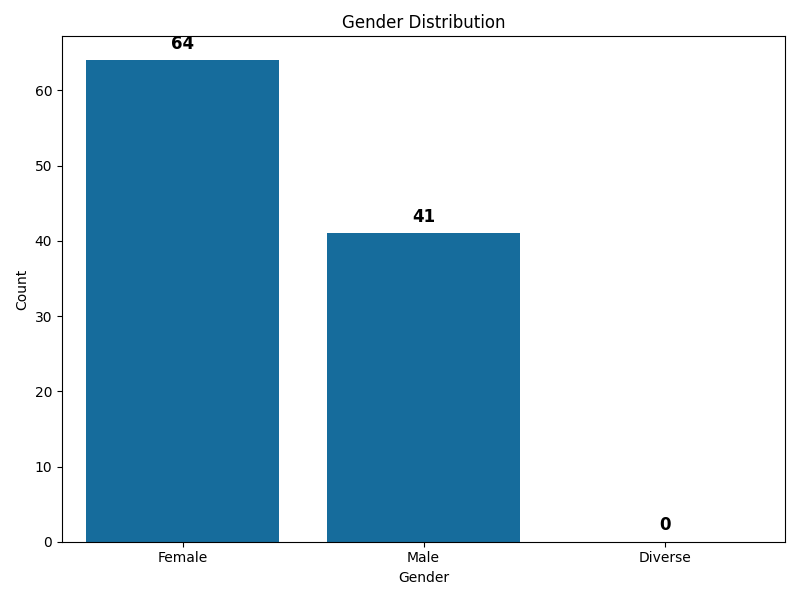
\includegraphics[width=0.6\textwidth]{./Bilder/gender_barplot.png}
  \caption{Geschlecht der Probanden}
  \label{fig:geschlecht}
\end{figure}

\begin{figure}[H]
    \centering
    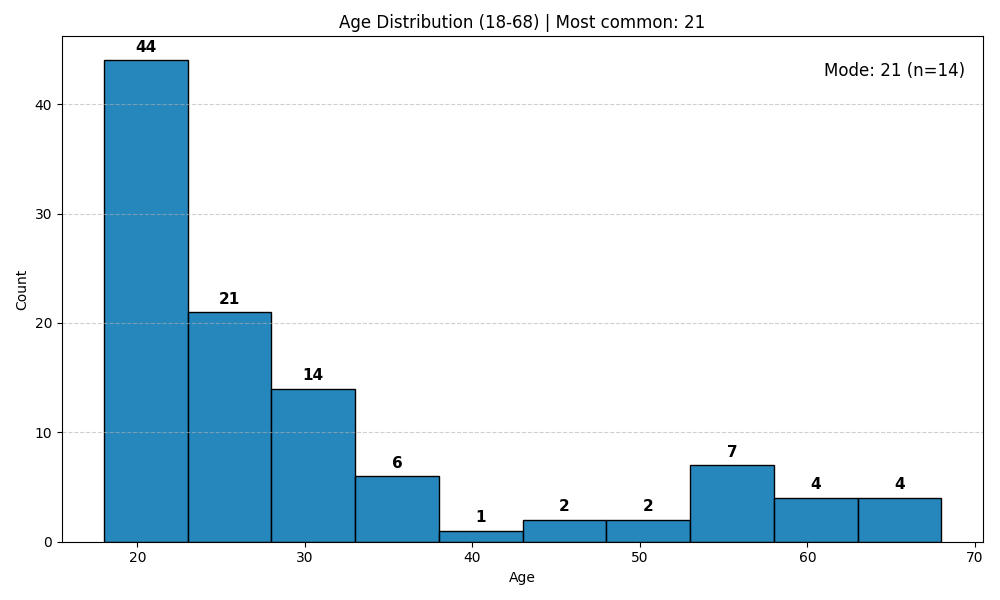
\includegraphics[width=0.6\textwidth]{./Bilder/age_histogram.png}
    \caption{Altersverteilung der Probanden}
    \label{fig:altersverteilung}
\end{figure}

\begin{figure}[H]
    \centering
    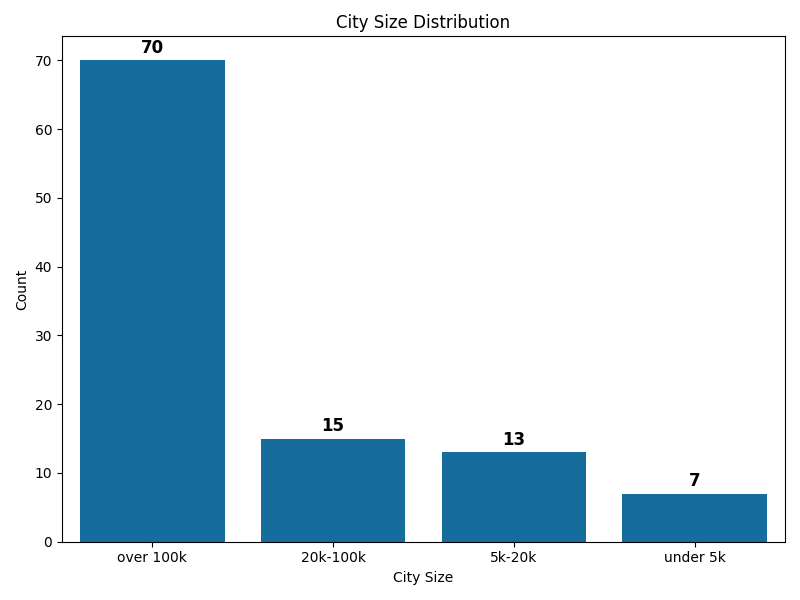
\includegraphics[width=0.6\textwidth]{./Bilder/city_size_barplot.png}
    \caption{Einwohneranzahl der Heimatstadt}
    \label{fig:einwohneranzahl}
\end{figure}

\begin{figure}[H]
    \centering
    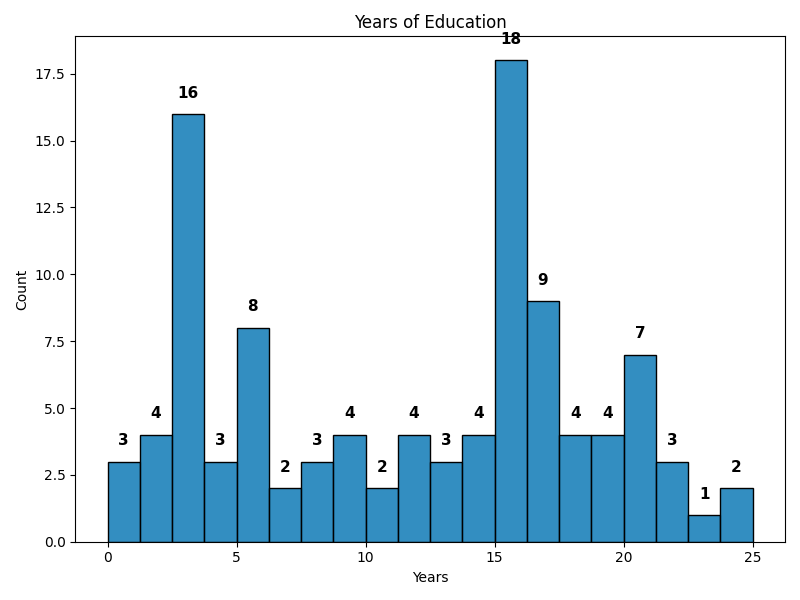
\includegraphics[width=0.6\textwidth]{./Bilder/education_histogram.png}
    \caption{Bildungsjahre der Probanden}
    \label{fig:bildungsjahre}
\end{figure}

\begin{figure}[H]
    \centering
    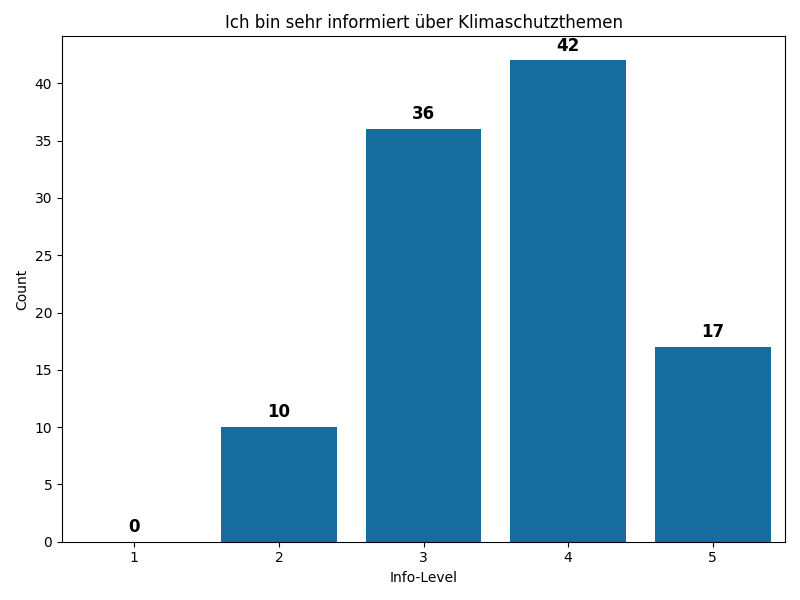
\includegraphics[width=0.6\textwidth]{./Bilder/info_klima_barplot.png}
    \caption{Vorkenntnisse über den Klimawandel}
    \label{fig:vorkenntnisse}
\end{figure}

\begin{figure}[H]
    \centering
    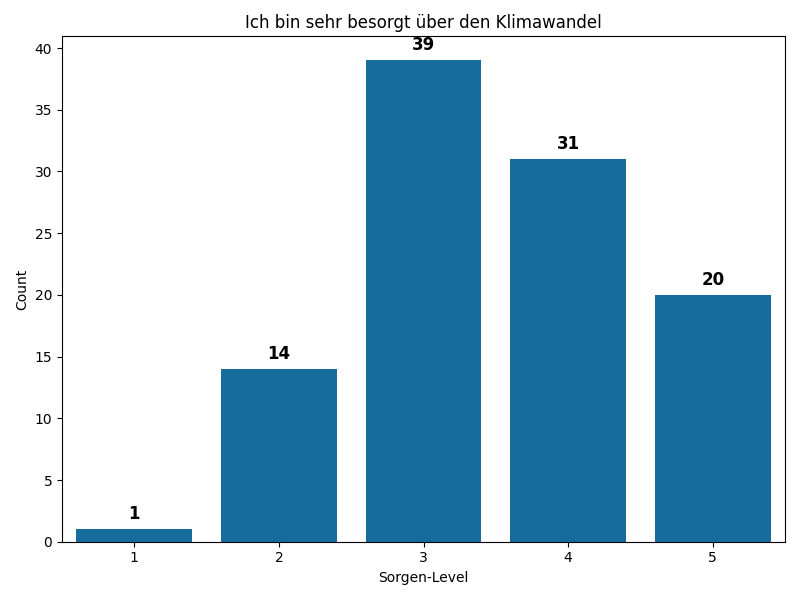
\includegraphics[width=0.6\textwidth]{./Bilder/sorgen_klima_barplot.png}
    \caption{Besorgnis über den Klimawandel}
    \label{fig:besorgnis}
\end{figure}

\end{document}
